%% Final Year Project Report Template
%% University of Sussex - School of Engineering and Informatics
%% Based on standard UK academic report format

\documentclass[12pt,a4paper]{article}

%% ============ PACKAGES ============
\usepackage[utf8]{inputenc}
\usepackage[T1]{fontenc}
\usepackage{mathptmx}  % Times New Roman font
\usepackage[margin=2.5cm]{geometry}
\usepackage{setspace}
\usepackage{graphicx}
\usepackage{float}
\usepackage{caption}
\usepackage{subcaption}
\usepackage{booktabs}
\usepackage{longtable}
\usepackage{array}
\usepackage{multirow}
\PassOptionsToPackage{hyphens}{url}
\usepackage{hyperref}
\usepackage{xurl}
\usepackage{xcolor}
\usepackage{listings}
\usepackage{fancyhdr}
\usepackage{titlesec}
\usepackage{tocloft}
\usepackage{parskip}
\usepackage{enumitem}
\usepackage{amsmath}
\usepackage{amssymb}

%% ============ CONFIGURATION ============
\onehalfspacing
\setlength{\emergencystretch}{3em}
\Urlmuskip=0mu plus 1mu\relax

% Word count automation (requires --shell-escape)
% Run: pdflatex --shell-escape Final_Report.tex
%
% === TEXCOUNT EXCLUSION DIRECTIVES ===
% Per university policy, the following are NOT counted:
% bibliography, footnotes, appendices, abstracts, figure legends, tables, acknowledgements
%TC:envir figure 0 0      % exclude figure environments (captions = figure legends)
%TC:envir table 0 0       % exclude table environments
%TC:envir tabular 0 0     % exclude tabular content
%TC:envir lstlisting 0 0  % exclude code listings
\immediate\write18{texcount -inc -sum -1 -q Final_Report.tex > wordcount.txt}
\newread\wordcountfile
\openin\wordcountfile=wordcount.txt
\ifeof\wordcountfile
    \newcommand{\wordcount}{[Run with --shell-escape]}
\else
    \read\wordcountfile to \wordcount
\fi
\closein\wordcountfile

% Hyperlink styling
\hypersetup{
    colorlinks=true,
    linkcolor=black,
    filecolor=black,
    urlcolor=blue,
    citecolor=black,
    pdfauthor={Duncan Law},
    pdftitle={AI-Powered Dynamic Narrative System for RPGs},
}

% Code listing style
\lstdefinestyle{gdscript}{
    backgroundcolor=\color{gray!10},
    basicstyle=\ttfamily\small,
    breakatwhitespace=false,
    breaklines=true,
    captionpos=b,
    commentstyle=\color{green!60!black},
    keywordstyle=\color{blue},
    stringstyle=\color{orange},
    numbers=left,
    numberstyle=\tiny\color{gray},
    numbersep=5pt,
    frame=single,
    framesep=5pt,
    xleftmargin=15pt,
    tabsize=4,
    showspaces=false,
    showstringspaces=false,
}
\lstset{style=gdscript}

% Header and footer
\setlength{\headheight}{14.5pt}
\pagestyle{fancy}
\fancyhf{}
\fancyhead[L]{\leftmark}
\fancyhead[R]{\thepage}
\renewcommand{\headrulewidth}{0.4pt}

% Section formatting
\titleformat{\section}{\normalfont\Large\bfseries}{\thesection}{1em}{}
\titleformat{\subsection}{\normalfont\large\bfseries}{\thesubsection}{1em}{}
\titleformat{\subsubsection}{\normalfont\normalsize\bfseries}{\thesubsubsection}{1em}{}

% Table of contents formatting
\renewcommand{\cftsecleader}{\cftdotfill{\cftdotsep}}

%% ============ DOCUMENT INFO ============
\newcommand{\reporttitle}{AI-Powered Dynamic Narrative System for RPGs}
\newcommand{\authorname}{Duncan Law}
\newcommand{\candidatenumber}{281967}
\newcommand{\degreecourse}{BSc Digital Media and Games Computing}
\newcommand{\department}{School of Engineering and Informatics}
\newcommand{\university}{University of Sussex}
\newcommand{\supervisor}{Dr Dan Creed}
\newcommand{\submissionyear}{2026}
% Note: \wordcount is now auto-generated above (requires --shell-escape)

%% ============ DOCUMENT START ============
\begin{document}

%% ============ COVER PAGE ============
\begin{titlepage}
    \centering
    \vspace*{2cm}

    {\Large \textbf{\university}}\\[0.5cm]
    {\large \department}\\[2cm]

    {\LARGE \textbf{G5038: Individual Project}}\\[0.5cm]
    {\Large Final Report}\\[2cm]

    {\Huge \textbf{\reporttitle}}\\[2cm]

    \begin{tabular}{rl}
        \textbf{Author:} & \authorname \\[0.3cm]
        \textbf{Candidate Number:} & \candidatenumber \\[0.3cm]
        \textbf{Degree Course:} & \degreecourse \\[0.3cm]
        \textbf{Supervisor:} & \supervisor \\[0.3cm]
        \textbf{Year of Submission:} & \submissionyear \\[0.3cm]
        \textbf{Word Count:} & \wordcount \\[0.3cm]
        \multicolumn{2}{p{12cm}}{\small\textit{Word count excludes: bibliography, footnotes/endnotes, appendices, abstract/summary, figure legends, tables, and acknowledgements, per University of Sussex assessment policy.}} \\
    \end{tabular}

    \vfill

    
\includegraphics[width=0.26\textwidth]{image/Interim-Report_281967.pdf-0-0.png}

    \vfill
\end{titlepage}

%TC:ignore
%% ============ STATEMENT OF ORIGINALITY ============
\newpage
\section*{Statement of Originality}
\addcontentsline{toc}{section}{Statement of Originality}

This report is submitted as part requirement for the degree of \degreecourse{} at the \university{}. It is the product of my own labour except where indicated in the text. The report may be freely copied and distributed provided the source is acknowledged.

I hereby \textbf{give} permission for a copy of this report to be loaned out to students in future years.

\vspace{2cm}

\noindent\textbf{Signature:} \underline{\hspace{6cm}}

\vspace{1cm}

\noindent\textbf{Date:} \underline{\hspace{6cm}}
%TC:endignore

%TC:ignore
%% ============ ACKNOWLEDGEMENTS ============
\newpage
\section*{Acknowledgements}
\addcontentsline{toc}{section}{Acknowledgements}

I would like to thank my supervisor, Dr Dan Creed, for his guidance and support throughout this project. His feedback during our regular meetings helped shape both the technical direction and the critical analysis presented in this report.

On a personal note, I am deeply grateful to the late Sita Chan. Although she tragically passed away in 2013, her enduring music provided the essential soundtrack that kept me focused and comforted during countless late-night coding and debugging sessions.

Finally, this project has been a personal reminder of the importance of balance. The process of building a game that critiques relentless productivity and blind optimism naturally prompted reflection on those same values in my own approach to work. I hope that message resonates with anyone who plays it.
%TC:endignore

%TC:ignore
%% ============ SUMMARY ============
\newpage
\section*{Summary}
\addcontentsline{toc}{section}{Summary}

This project investigates the integration of Large Language Models (LLMs) into interactive narrative games through the development of ``Glorious Deliverance Agency 1,'' a 2D text-based RPG built in the Godot engine. The game employs a bespoke pipeline architecture where the LLM operates within explicit developer-defined constraints to generate dynamic narrative content whilst maintaining thematic coherence.

The implementation features a multi-provider AI architecture supporting Gemini, OpenRouter, Ollama, and Mock providers, enabling development flexibility and cost management. A three-layer context-management system balances narrative coherence with token efficiency, whilst the ``Reality vs. Positive Energy'' thematic framework constrains AI generation to produce satirically appropriate content.

Key technical contributions include the Strategy pattern for provider abstraction, an EventBus for cross-module communication, and defensive multi-stage response parsing to handle non-deterministic AI outputs. The project demonstrates that bespoke pipeline approaches can successfully integrate LLM-generated content into playable games, providing practical insights for developers considering similar integrations.

Functional testing across approximately one hundred narrative generations achieved fewer than ten percent requiring intervention due to tonal inconsistency, meeting the defined success criteria. The comparative analysis identifies concrete trade-offs between bespoke pipelines and world model approaches regarding control versus emergence, development complexity versus scope, and predictability versus novelty.
%TC:endignore

%% ============ TABLE OF CONTENTS ============
\newpage
\tableofcontents

%% ============ MAIN CONTENT ============
\newpage
\setcounter{page}{1}
\pagenumbering{arabic}

%% ============ SECTION 1: INTRODUCTION ============
\section{Introduction}

\subsection{Project Aims and Objectives}

I am developing ``Glorious Deliverance Agency 1,'' a 2D text-based RPG built in the Godot engine that uses Large Language Model (LLM) integration to generate dynamic narrative content. The game places players as a reluctant hero in a dysfunctional team, whose attempts to save the world with ``positive energy'' only accelerate its destruction through a darkly comedic narrative that responds to their choices in real-time.

Traditional RPG narratives rely on pre-scripted dialogue trees and fixed storylines, limiting replayability and player agency. While LLMs offer the potential for dynamic content generation, integrating them into games presents significant challenges: maintaining narrative coherence over extended play sessions, ensuring thematic consistency with authorial intent, and managing the practical constraints of API latency and token costs. I investigated whether a carefully structured ``bespoke pipeline'' approach, where the LLM operates within explicit developer-defined constraints, can address these challenges to produce a playable, thematically coherent RPG experience. My central research question is therefore: to what extent can a text-based LLM, integrated as a controlled component within a traditional game engine, generate coherent and thematically consistent narrative content for an interactive RPG?

My primary aim is supported by three foundational pillars. The first pillar, Technical Development, involved the design and implementation of a functional AI-driven 2D RPG narrative system. The game features dynamically generated storylines and NPC dialogue, where ``dynamically'' refers to the real-time generation of narrative content based on the current game state and player choices, moving beyond traditional pre-scripted narratives. My technical focus was on enabling emergent, non-linear story paths while maintaining narrative coherence over extended gameplay sessions through a three-layer context-management system (detailed in Appendix C: GDD, Section 7.2).

The second pillar, Thematic Execution, centres on creating a satirical allegory exploring the conflict between ``positive energy'' ideology and the concept of Void Entropy. The core gameplay mechanics, including the Reality vs. Positive Energy system and the Prayer System, deliberately subvert conventional RPG expectations (see Appendix C: GDD, Sections 4.2--4.3 for detailed mechanics). I have embedded these thematic concepts directly into the AI's prompt engineering, ensuring that generated content aligns with my project's darkly satirical tone rather than producing generic positive outcomes.

The third pillar, Critical Analysis, involved producing a comparative analysis of my ``bespoke pipeline'' methodology against the theoretical ``world model'' paradigm. I examined architectural trade-offs between fine-grained developer control and emergent simulation capabilities, explored the shifting role of the developer from systems architect to high-level director, and assessed the practical feasibility of each approach based on my direct implementation experience.

To ensure these aims remain achievable within the project's constraints, I have defined concrete success criteria. For Technical Development, success means producing a functional prototype that can generate coherent narrative content across multiple consecutive scenes without critical errors, with measurable metrics including API response latency under five seconds and successful context preservation across save/load cycles. For Thematic Execution, success means the AI consistently generates content that aligns with the ``Reality vs. Positive Energy'' framework during functional testing, with fewer than one in ten generations requiring manual intervention due to tonal inconsistency. For Critical Analysis, success means producing a structured comparison document that draws on my direct implementation experience to identify at least three concrete architectural trade-offs between bespoke pipelines and world-models. These criteria are deliberately scoped to be demonstrable through functional testing rather than requiring extensive user studies.

\subsection{Justification of Technical and Narrative Choices}

I selected the Godot 4.x engine as my development platform due to its open-source nature and scene-node architecture, which facilitates the construction of UI-heavy applications suitable for narrative-driven games. The engine's support for both C\# and GDScript provides flexibility for integrating external AI services through custom modules, while its lightweight footprint ensures rapid iteration during development.

I employed Gemini-2.5-flash as my primary LLM provider, selected based on latency and cost performance, convenient API and toolchain integration, and sufficient context length to support extended interactive narrative sessions (Google, 2025). Actual available context and performance vary by model and configuration; therefore, my final evaluation criteria are based on functional test results within my project's specific scenario, including long-term narrative consistency, response time, and cost monitoring, rather than pure specification comparisons. This approach ensures my assessment reflects practical implementation requirements rather than theoretical capabilities.

My narrative framework, centred on the thematic tension between ``Reality'' and ``Positive Energy,'' serves a dual purpose. First, it provides a testbed for evaluating the AI's capacity to maintain thematic coherence within a defined conceptual space. Second, the deliberately ironic and darkly satirical tone presents a challenge for the model's stylistic consistency, testing whether the system can generate content that aligns with specific tonal and thematic constraints rather than producing generic narrative outputs. I designed this approach to explore how effectively a bespoke pipeline can maintain authorial intent within AI-generated content.

\subsection{Target User Group and Scope}

During development, I served as the primary user, functioning as the sole tester in a functional testing capacity. This reflects my project's nature as a research prototype investigating AI-driven narrative generation, where the unpredictable nature of LLM outputs necessitates thorough internal validation before external exposure.

The intended eventual audience for ``Glorious Deliverance Agency 1'' is detailed in Appendix C: Game Design Document, Section 1.5 (Target Audience), which defines both primary and secondary user groups. The game's dark satirical tone and thematic content make it unsuitable for younger audiences; a mature content advisory would be appropriate for any public release.

For the purposes of this academic project, however, I limited the scope to demonstrating technical feasibility and thematic coherence through developer-led functional testing. I did not plan formal user studies with external participants at this stage, as the ethical framework I outline in Section 3 required first establishing confidence in the system's output behaviour.

\subsection{Expected Findings and Achievements}

By the project's completion, I demonstrated that a bespoke pipeline architecture can successfully integrate LLM-generated content into a playable RPG while maintaining thematic coherence. Specifically, I showed that my three-layer context-management system preserves narrative consistency across extended play sessions, that the ``Reality vs. Positive Energy'' framework effectively constrains AI generation to produce satirically appropriate content, and that the multi-provider architecture enables practical development within budget constraints. The comparative analysis identified concrete trade-offs between bespoke pipelines and world model approaches, providing insights for developers considering similar integrations. While the prototype did not achieve commercial-quality polish, it successfully demonstrates the viability of controlled LLM integration for narrative games.

\subsection{Report Structure}

This report is organised as follows. Section 2 reviews relevant literature on AI in games, LLM integration, and narrative coherence, establishing the theoretical foundation for my approach. Section 3 addresses professional and ethical considerations, particularly regarding AI-generated content. Section 4 presents my project specification and methodology, including success criteria and evaluation plans. Section 5 provides an overview of the system design through architectural diagrams. Section 6 reflects on project management, discussing planning approaches and lessons learned. Section 7 details the design decisions and patterns employed in my implementation. Section 8 describes the implementation process, including challenges encountered and solutions developed. Section 9 covers my testing strategy and results. Section 10 evaluates the project against original requirements and provides a comparative analysis of bespoke pipelines versus world-models. Finally, Section 11 concludes with a summary of achievements, lessons learned, and directions for future work.

%% ============ SECTION 2: BACKGROUND ============
\section{Background and Literature Review}

\subsection{AI in Games and Generative Narrative Systems}

The emerging field of generative narrative systems, increasingly powered by Procedural Content Generation (PCG) and Large Language Models (LLMs), treats story not as a fixed script but as a co-creative space shaped by both the player and the system in real-time (Sun et al., 2023; Al-Surayhi et al., 2025). In ``Glorious Deliverance Agency 1,'' I positioned the LLM as the ``story director'' itself, orchestrating scene transitions, generating contextual NPC responses, and determining narrative consequences based on player choices and current game state.

The ``storylet'' concept, a small, self-contained narrative unit with defined prerequisites and effects that the system sequences dynamically based on game state (Short, 2019), directly shaped my architecture. I adopted this pattern in my AIManager, which generates discrete narrative ``beats'' triggered by specific game conditions, each producing defined effects on the game state.

The central engineering challenge was the ``controllability problem'': balancing AI freedom to surprise players whilst maintaining thematic coherence (Balint and Bidarra, 2023; AlHussain and Azmi, 2021). I addressed this through a multi-layered context model: a static ``world bible'' layer establishing firm thematic guardrails within which the LLM generates content guided by short-term event memory and summarised long-term history.

\subsection{Large Language Models for Interactive Narratives}

Researchers have demonstrated that LLMs can generate context-aware NPC dialogue aligned with character personas (Chen, 2025) and produce procedural quest descriptions comparable to human-authored content (Värtinen et al., 2022). These results came from prompt engineering rather than model re-training. My AIManager constructs prompts that embed persona definitions for each NPC, ensuring Saint Gloria's toxic positivity, Sir Donkey's delusional heroism, and ARK's obsessive bureaucracy maintain distinct voices (Yang et al., 2024).

The distinction between ``world model'' and ``bespoke pipeline'' approaches was critical. World models, exemplified by Park et al.'s (2023) ``Generative Agents'', simulate entire environments from the ground up with agents possessing memory, reflection, and planning capabilities. The bespoke pipeline integrates an LLM as one component within a traditional game engine, grounding it with structured game state data (Góngora et al., 2025). In my implementation, the Godot engine maintains authoritative game state whilst the LLM operates as a content generation service.

World models promise emergence and player freedom but face limitations in ensuring consistent narratives and require immense computational cost (Yang et al., 2024). Bespoke pipelines offer authorial control but at the cost of emergent possibility (Góngora et al., 2025). Wan et al. (2025) confirmed that making LLMs adhere to complex constraints requires continuous architectural attention.

\subsection{Bespoke Pipelines vs. World-Model Approaches}

Here I contextualise my architectural choice before the implementation chapters that follow. A bespoke pipeline integrates a general-purpose LLM as a component within a traditional game engine, in my case, Godot plus an LLM API, enabling controlled state management and narrative guidance through explicit developer-defined constraints. When I began researching alternatives, I found that world model approaches pursue end-to end generation of entire interactive environments, but current publicly accessible systems remain insufficient for a single-developer project of this scope (Parker-Holder and Fruchter, 2025). The bespoke pipeline was therefore not merely a preference but a practical necessity. My implementation reflects this clearly: the Godot engine handles all game logic, state persistence, and UI rendering, whilst the LLM API is invoked only for narrative text generation, with clearly defined input schemas and output formats. This separation allowed me to develop, test, and debug each layer independently.

\subsection{Coherence and Evaluation in AI-Generated Narratives}

Narrative coherence, the logical and causal consistency of events, character behaviours, and world stability, is where generative systems tend to fail (Yi et al., 2025). For my project, coherence failures would manifest as NPCs forgetting conversations, contradicting plot points, or shifting from satirical to sincere tone.

For a single-developer project generating non-deterministic outputs, I concluded that functional testing was more appropriate than automated benchmarking (Wan and Ma, 2025; El Boudouri et al., 2025). I adopted a protocol built around three questions: did the AI maintain the thematic framework? Did content align with the dark satirical tone? Did the context-management system prevent contradictions?

The memory management literature informed my three-layer context model (Yi et al., 2025; Park et al., 2023), with specific token allocations detailed in Appendix C: GDD, Section 7.2.

\subsection{Runtime Constraints and Practical Considerations}

Latency significantly impacts immersion in interactive narratives (Schomay, 2024; Juliani, 2025). I addressed this through the Strategy pattern in my AIManager, enabling runtime provider switching depending on performance conditions (documented in Appendix C: GDD, Section 7.1).

Token budgets required careful management. Rather than feeding entire conversation histories into prompts, production systems use hierarchical summarisation, Retrieval-Augmented Generation, and automated pruning (Sridi, 2025; Anthropic, 2025; DZone, 2024). I implemented token monitoring in my AIManager, logging input and output counts per API call.
This was also consistent with how GitHub Copilot and Claude handle long contexts in practice: layered summaries and relevance filtering instead of replaying full transcripts. That industry pattern directly influenced my three-layer memory architecture (static rules, short-term events, long-term summaries).

For content safety, I constrained the input space at the UI level, requiring players to choose from predefined buttons rather than type freely (Buongiorno et al., 2024; O'Brien, 2024). This eliminated unexpected prompt inputs before they reached the AI.

Juliani's (2025) warning about ``infinite trash'' and Vidler and Walsh's (2025) findings on LLM statistical biases informed my approach: the AI needed explicit directional constraints about narrative goals, not just content restrictions. For a narrative game built around ironic inversion, this was essential.

\subsection{Thematic Control and Values-Based Systems}

Juliani (2025) identifies ``mode collapse'' in LLM generation: models prompted for a specific genre over-rely on statistically common surface markers, producing repetitive content. To avoid this, I designed an explicit values-based system (see Appendix C: GDD, Section 4.2) where every player choice quantifiably impacts ``Reality'' and ``Positive Energy'' stats, which feed directly into AI prompts to modulate tone and direction. This transforms the theme into a measurable, directive principle rather than a static premise.

This approach also resolved the ``infinite trash'' problem (Juliani, 2025). Rather than aiming for complete narrative freedom, I framed player agency within a core ironic loop: positive intentions systematically convert into negative outcomes. The Prayer System embodies this (Appendix C: GDD, Section 4.3), balancing dynamic generation with authorial control.

\subsection{Research Gaps and Implications for My Project}

Research either examines theoretical world-models at scale (Parker-Holder and Fruchter, 2025) or general LLM integration without tight thematic constraints (OpenAI, 2023; Pichai and Hassabis, 2023). What is missing is a practical account of the engineering effort, prompt complexity, and architectural decisions required to maintain author-driven thematic control within a bespoke pipeline.

My original contributions include: the three-layer context architecture balancing token budgets with narrative continuity; the values-based generation control system enforcing thematic alignment through quantified game stats; the functional testing framework for evaluating thematic coherence in non-deterministic outputs; and the comparative analysis contributing grounded empirical observations to world model discourse.

This literature review directly shaped my architectural decisions. The storylet concept informed my modular narrative generation approach. The memory management research informed my three-layer context system. The mode collapse problem motivated my values-based prompt control. The bespoke pipeline versus world model distinction provided the conceptual framework for understanding why the constraints I imposed were necessary.

%% ============ SECTION 3: PROFESSIONAL CONSIDERATIONS ============
\section{Professional Considerations and Ethical Framework}

Building this project required me to consider professional and ethical responsibilities carefully, guided by the British Computer Society (BCS) Code of Conduct. Having studied relevant modules at the University of Sussex, I can claim competence in the technical areas this project addresses (BCS Code of Conduct 2.a, 2.b). All claims and referenced works are properly documented to avoid misrepresentation (BCS Code of Conduct 2.f).

\subsection{Primary Risk: AI Content Generation}

The key ethical insight for my project is that the primary risk is not traditional data privacy concerns, but rather the potential for generative AI to produce unexpected or inappropriate content. Given my project's deliberately dark satirical narrative framework, there exists a genuine possibility that the AI could generate content that crosses boundaries of acceptability. At this stage of development, it is not possible to predict with certainty what content the AI might generate, which is precisely why formalised user testing with external participants is not appropriate until the system's output behaviour has been thoroughly validated.

\subsection{Functional Testing as Ethical Safeguard}

I adopted functional testing as both a methodological approach and an ethical safeguard, serving as the sole tester to observe what content the AI generates and whether it remains within acceptable boundaries. This is an ongoing process, as the nondeterministic nature of LLM outputs means each generation session may produce different results.

The following categories constitute definitive red lines that would trigger immediate testing termination and require architectural intervention before resumption. Content depicting or encouraging real-world violence, self-harm, or suicide represents the first and most critical red line; while my game's satirical framework permits dark humour about abstract concepts like ``entropy,'' any generation promoting genuine harm to individuals is unacceptable. The second red line concerns discriminatory content targeting protected characteristics; the satire must critique systems and behaviours rather than denigrate individuals based on race, gender, religion, disability, or other protected attributes. The third red line addresses sexually explicit material, which is entirely outside my project's thematic scope and would indicate a fundamental failure of prompt constraints. The fourth red line involves content that constitutes legal liability, such as defamatory statements about real individuals or institutions, or content that could reasonably be interpreted as incitement.

\subsection{Control Measures}

My primary mitigation strategy is embedded in the core UI design: the system uses predefined button choices for player interaction rather than open-ended text input, significantly constraining the space of possible prompts sent to the AI. I explicitly considered and rejected voice input due to ethical concerns including the potential for inadvertently recording background conversations.

The Prayer System permits short text input as an ironic game mechanic but remains constrained by cooldown timers, templated prompt construction, and content filtering.

\subsection{Data Protection}

API keys are stored exclusively on my local machine within Godot's sandboxed user directory, excluded from version control. System logs capture AI prompts and responses for evaluation purposes, stored locally without personally identifiable information. When local Ollama models are used, all processing occurs on local hardware with no third-party data transmission.

These ethical considerations shaped my technical decisions throughout the project, particularly the choice to use button-based input rather than free text and the implementation of content filtering.

Having established the ethical framework guiding this project, Section 4 translates these commitments into a formal project specification and methodology.

%% ============ SECTION 4: PROJECT SPECIFICATION ============
\section{Project Specification and Methodology}

I built the system using the Godot 4.x game engine with a modular architecture employing singleton manager classes to provide globally accessible services. The system architecture, component specifications, and interface definitions are fully documented in Appendix C: Game Design Document, Sections 7.1--7.6.

My system employs a Strategy design pattern supporting multiple provider types (detailed in Appendix C: GDD, Section 7.1). This architecture enables development flexibility and cost management through provider switching.

As I identified in Section 2.5, effective context-management is critical for maintaining narrative coherence. I implemented a three-layer context model balancing narrative coherence with token efficiency (see Appendix C: GDD, Section 7.2 for complete specifications).

\begin{figure}[H]
    \centering
    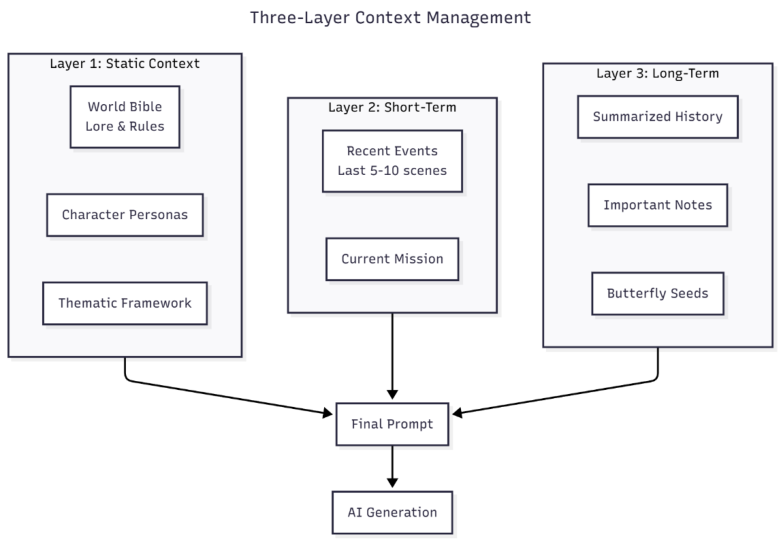
\includegraphics[width=0.85\textwidth]{image/Interim-Report_281967.pdf-8-0.png}
    \caption{Three-Layer Context Management Architecture. The diagram illustrates how static context, short-term context, and long-term memory are combined into a final prompt for AI generation.}
    \label{fig:context-management}
\end{figure}

I evaluated the project through functional testing focused on determining whether the system performed as intended across three key dimensions: technical functionality, thematic coherence, and player experience quality. The testing strategy and evidence plan are detailed in Appendix C: GDD, Section 5.

I defined success as achieving functional technical implementation where core systems operate reliably without critical errors, maintaining thematic coherence where AI-generated content consistently aligns with the established satirical framework, and demonstrating player experience potential where implemented mechanics exhibit qualities associated with engaging gameplay.

My evaluation assessed whether core systems operated correctly through direct testing. Key questions included: did the AI integration successfully generate narrative content? Did the provider switching mechanisms function reliably? Did the context-management system maintain state across extended sessions without errors? Did the game handle AI generation failures gracefully? I instrumented the AIManager to log performance metrics, including API latency and token consumption, enabling analysis of cost-effectiveness and responsiveness trade-offs between different AI providers. Implementation details for the testing infrastructure are documented in Appendix C: GDD, Section 5.1--5.2.

Functional testing determined whether AI-generated content aligned with my project's specific thematic intent. Did the system maintain the ``Reality vs. Positive Energy'' thematic framework consistently? Did the Prayer System reliably produce ironic, satirically appropriate outcomes rather than generic positive responses? Did my three-layer context model effectively prevent narrative contradictions and thematic drift across extended gameplay? As the functional tester, I made qualitative assessments of whether generated content served the artistic vision or undermined it.

While formal player testing with external participants was not appropriate at this development stage, my functional testing process evaluated whether the system generated content that could constitute an engaging player experience. Drawing on established game design frameworks, ``fun'' in this context comprises several elements: challenge (do player choices present meaningful dilemmas?), rules (are the game's systems comprehensible and consistent?), goals (does the narrative create clear objectives and progression?), and options (does the AI provide sufficiently varied choices?). I assessed whether the implemented features, dynamic narrative generation, state-based choice consequences, teammate interference systems, moral dilemmas, functioned not merely technically but also served to create an experience with these qualities.

My comparison to ``world model'' approaches remained purely theoretical, based on public documentation (Parker-Holder and Fruchter, 2025), focusing on architectural trade-offs rather than direct performance benchmarks. I drew on my implementation experience and functional testing observations from this bespoke pipeline to provide grounded insights into the practical implications of architectural choices.

My methodology assumed that a mock AI provider is sufficient for most UI and logic development. I acknowledge the inherent variability and non-determinism of LLM outputs, which presents a challenge for repeatable testing. I operated under a limited API budget, reinforcing the need for the Ollama and mock provider paths.

The third pillar of my project, the critical analysis, was conducted by comparing my ``bespoke pipeline'' methodology against the theoretical ``world model'' paradigm through conceptual and architectural analysis based on publicly available research documentation (Parker-Holder and Fruchter, 2025). This is not an empirical benchmark, as world model technologies are not publicly available for direct testing.

I drew from two primary sources: (a) my direct implementation experience and evaluation data from this project, which serves as a concrete example of a bespoke pipeline, and (b) the publicly available technical reports, research papers, and blog posts describing world model research such as Google's Genie project (Parker-Holder and Fruchter, 2025) and the underlying capabilities of large models from providers like OpenAI (OpenAI, 2023).

My comparison framework contrasted: (1) architectural trade-offs between the modular bespoke pipeline (Godot Engine + LLM API) offering fine-grained control and integrated world-models promising emergent scope; and (2) the shifting developer role from systems architect in bespoke approaches to high-level director in world model paradigms. This structured analysis provided grounded insights into the practical implications of architectural choices, drawing on my direct implementation experience.

Adopting this methodology proved essential for managing the inherent unpredictability of LLM-based systems. The spiral development approach allowed me to iteratively refine prompt engineering and context-management based on observed AI behaviour, whilst the multi-provider strategy ensured development continuity despite external API constraints.

With the methodology established, Section 5 presents the system design that emerged from applying it.

%% ============ SECTION 5: SYSTEM DESIGN ============
\section{System Design}

I have designed the system architecture to be modular and scalable, built around decoupled singleton manager components and purpose-built UI scene controllers. This separation of concerns is critical for managing non-deterministic AI components. Components communicate through clearly defined signal-based interfaces to minimise coupling while enabling complex AI feedback loops. Comprehensive technical specifications are documented in Appendix C: Game Design Document, Sections 7.1--7.6. The following diagrams provide a high-level overview of the architecture.

\begin{figure}[H]
    \centering
    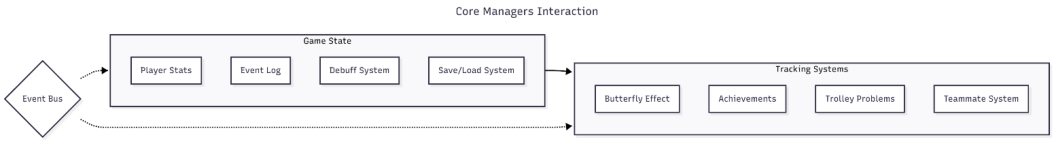
\includegraphics[width=0.8\textwidth]{image/Interim-Report_281967.pdf-10-0.png}
    \caption{Core Managers Interaction. The Event Bus facilitates communication between the Game State subsystem (Player Stats, Event Log, Debuff System, Save/Load System) and the Tracking Systems (Butterfly Effect, Achievements, Trolley Problems, Teammate System).}
    \label{fig:core-managers}
\end{figure}

\begin{figure}[H]
    \centering
    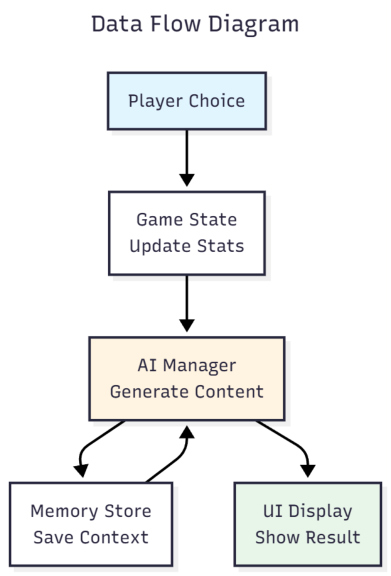
\includegraphics[width=0.8\textwidth]{image/Interim-Report_281967.pdf-10-1.png}
    \caption{Data Flow Diagram. Player choices trigger game state updates, which inform the AI Manager's content generation. Generated content is simultaneously stored in the memory system and displayed through the UI.}
    \label{fig:data-flow}
\end{figure}

\begin{figure}[H]
    \centering
    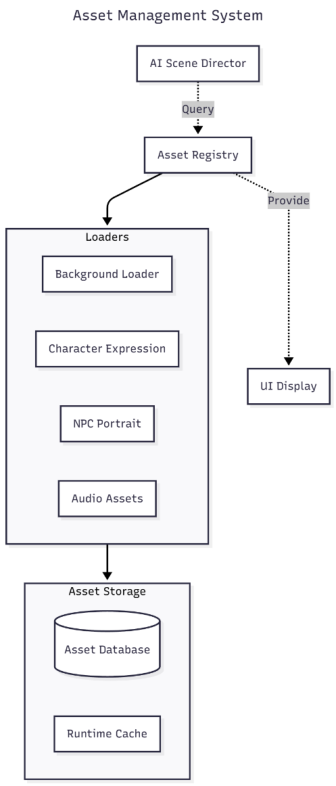
\includegraphics[width=0.8\textwidth]{image/Interim-Report_281967.pdf-10-2.png}
    \caption{Asset Management System. The AI Scene Director queries the Asset Registry to load appropriate backgrounds, character expressions, NPC portraits, and audio assets for display in the UI, with assets stored in a database and runtime cache.}
    \label{fig:asset-management}
\end{figure}

\begin{figure}[H]
    \centering
    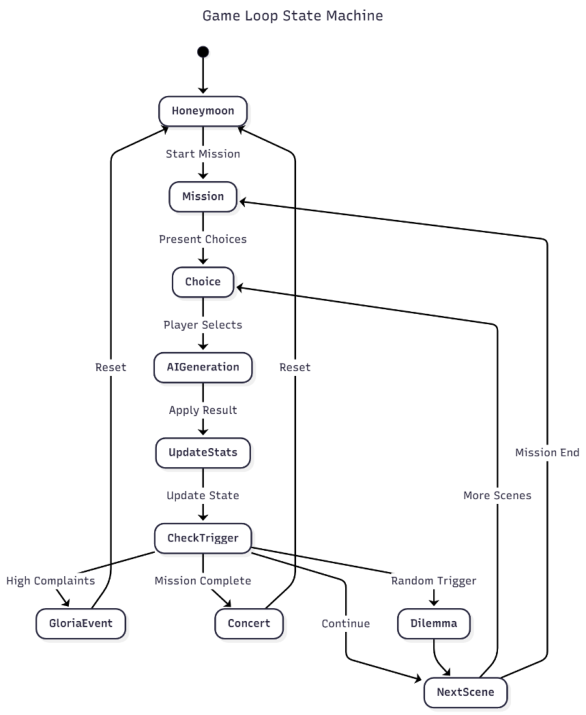
\includegraphics[width=0.8\textwidth]{image/Interim-Report_281967.pdf-11-0.png}
    \caption{Game Loop State Machine. The diagram shows the core gameplay flow from Honeymoon through Mission, Choice, AIGeneration, UpdateStats, and CheckTrigger states, with branching paths to special events (GloriaEvent, Concert, Dilemma) and scene transitions.}
    \label{fig:game-loop}
\end{figure}

\begin{figure}[H]
    \centering
    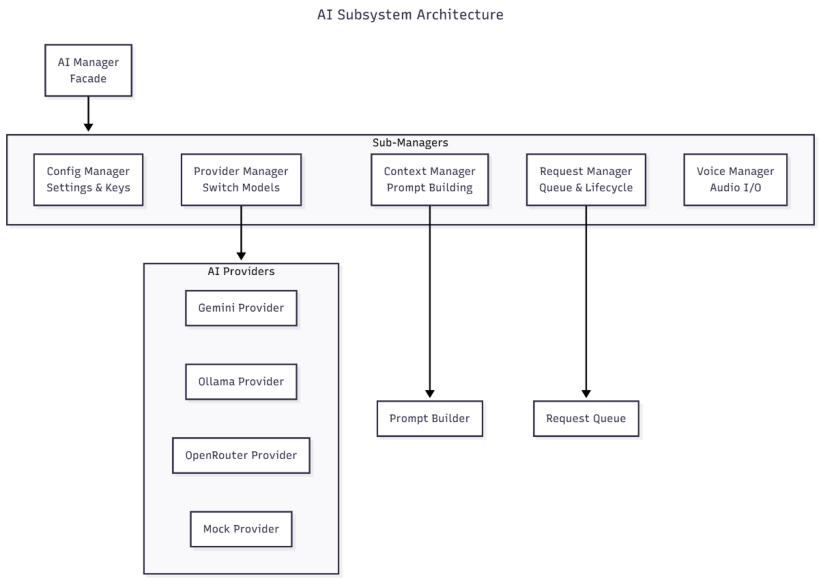
\includegraphics[width=0.8\textwidth]{image/Interim-Report_281967.pdf-11-1.png}
    \caption{AI Subsystem Architecture. The AI Manager Facade coordinates Sub-Managers (Config Manager, Provider Manager, Context Manager, Request Manager, Voice Manager), which interface with multiple AI Providers (Gemini, Ollama, OpenRouter, Mock) through a unified Prompt Builder and Request Queue.}
    \label{fig:ai-subsystem}
\end{figure}

\begin{figure}[H]
    \centering
    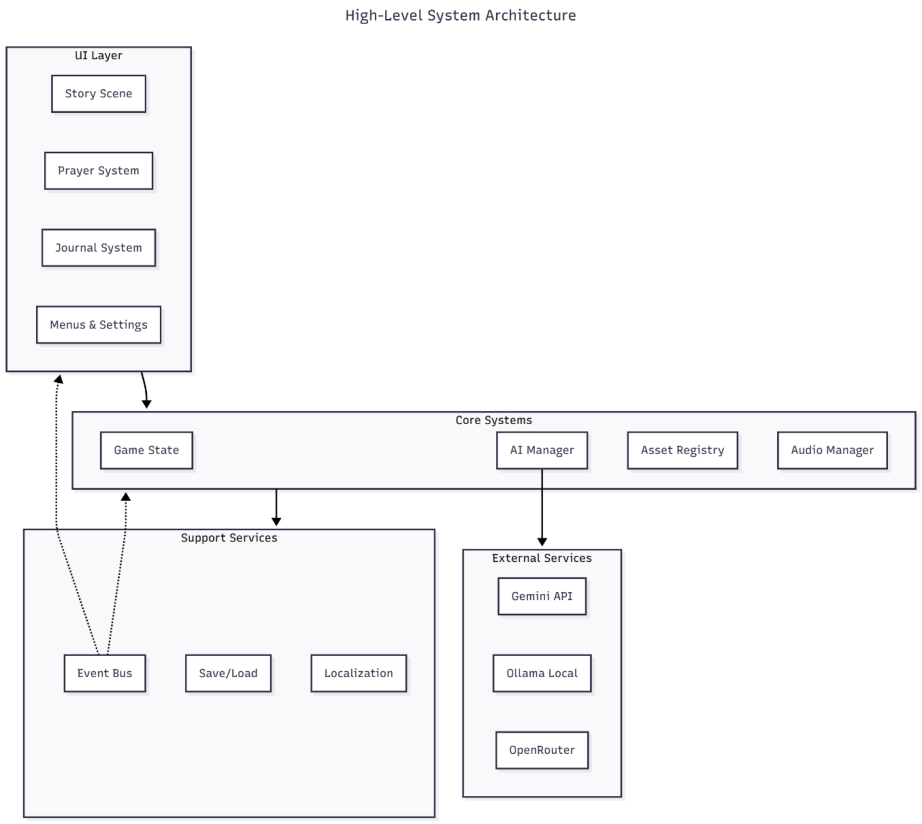
\includegraphics[width=0.8\textwidth]{image/Interim-Report_281967.pdf-12-0.png}
    \caption{High-Level System Architecture. The UI Layer (Story Scene, Prayer System, Journal System, Menus and Settings) interfaces with Core Systems (Game State, AI Manager, Asset Registry, Audio Manager), Support Services (Event Bus, Save/Load, Localisation), and External Services (Gemini API, Ollama Local, OpenRouter).}
    \label{fig:high-level-arch}
\end{figure}

This modular architecture proved essential for managing the complexity of AI integration. The clear separation between deterministic game logic and non-deterministic AI generation enabled independent development and testing of each layer, whilst the signal-based communication patterns facilitated debugging when unexpected AI outputs propagated through the system.

These design boundaries enabled the development workflow described in Section 6, where provider switching and isolated component testing were essential for progress.

%% ============ SECTION 6: PROJECT MANAGEMENT ============
\section{Project Management Reflection}

I organised the project into five phases: Foundation, Planning, Core Development, Integration, and Finalisation, illustrated in Figure~\ref{fig:gantt-chart}. The multi-provider architecture strategy, planning for Gemini, OpenRouter, Ollama, and Mock providers from the outset, proved essential as both a technical feature and a project management strategy, enabling development to continue when I encountered API rate limiting issues. This defensive planning approach was critical for working with non-deterministic AI systems where outputs cannot be fully predicted in advance.
I also built explicit buffer time between phases; this reserve absorbed unexpected response parsing issues during Core Development without causing a full schedule slip. In addition, I changed prompt engineering from a fixed two-week milestone into an ongoing parallel track, because output instability and rate-limit constraints required repeated template refinement across the whole implementation period.

\begin{figure}[H]
    \centering
    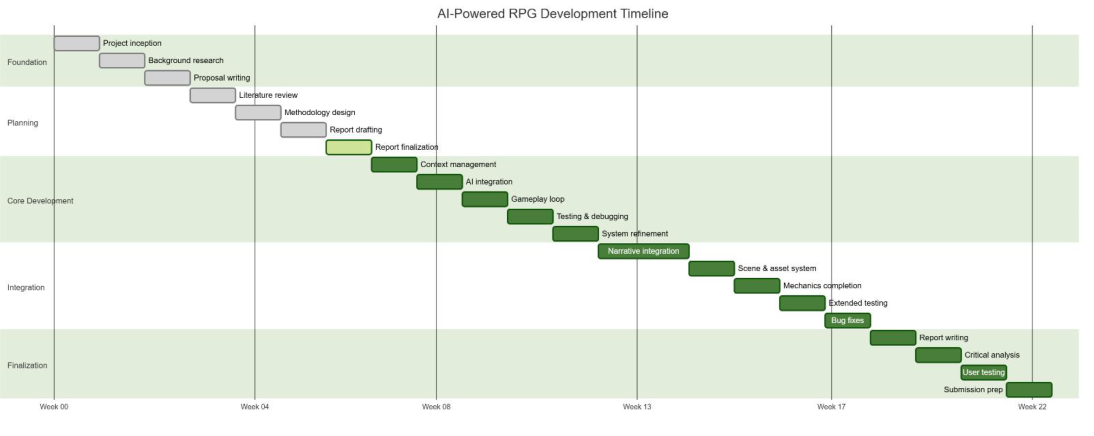
\includegraphics[width=0.9\textwidth]{image/Interim-Report_281967.pdf-13-0.png}
    \caption{AI-Powered RPG Development Timeline (Gantt Chart). The timeline spans from Week 00 to Week 22, organised into five phases: Foundation (project inception, background research, proposal writing), Planning (literature review, methodology design, report drafting), Core Development (context-management, AI integration, gameplay loop, testing), Integration (scene and asset system, mechanics completion, extended testing), and Finalisation (bug fixes, report writing, critical analysis, user testing, submission preparation).}
    \label{fig:gantt-chart}
\end{figure}

Section 7 examines the design decisions this planning made possible.

%% ============ SECTION 7: DESIGN ============
\section{Design}

In this section I document the architectural decisions that shaped my implementation, explaining not merely what I built but why I made specific design choices given the unique challenges of integrating non-deterministic AI components into a real-time game engine.

\subsection{Architectural Philosophy: Separation of Deterministic and Non-Deterministic Systems}

The fundamental design challenge I faced was integrating inherently unpredictable LLM outputs into a game engine that expects deterministic behaviour. Traditional game architectures assume that given the same inputs, systems will produce the same outputs; LLMs violate this assumption fundamentally. My architectural response was to establish a clear boundary between the deterministic game logic layer and the non-deterministic AI generation layer, with carefully designed interfaces mediating between them.

I organised my codebase into three primary layers. The Core Systems Layer contains singleton managers responsible for game state, audio, asset-management, and event coordination. These systems operate deterministically and maintain authoritative game state. The AI Integration Layer encapsulates all LLM-related functionality behind a facade pattern, presenting a consistent interface regardless of which AI provider is active. The UI Layer implements scene-specific controllers that react to both game state changes and AI-generated content, rendering the player experience.

\subsection{Design Patterns and Their Justifications}

I employed several established design patterns, each chosen to address specific architectural challenges.

For dependency management, rather than passing dependencies through constructor chains or using global singletons directly, I implemented a Service Locator that manages access to all global services. This decision emerged from practical necessity during development; as the project grew, I found myself frequently refactoring constructor signatures when adding new dependencies. The ServiceLocator provides typed accessor methods such as \texttt{get\_game\_state()} and \texttt{get\_ai\_manager()}, enabling IDE autocompletion whilst maintaining loose coupling between components (see \texttt{service\_locator.gd:54--95} for implementation).

For AI provider management, the multi-provider architecture uses the Strategy pattern to enable runtime switching between Gemini, OpenRouter, Ollama, and Mock providers. Each provider implements the \texttt{AIProviderBase} interface, which defines \texttt{send\_request()}, \texttt{cancel\_request()}, and \texttt{is\_configured()} methods. This design proved essential during development; when I encountered rate limiting on the Gemini API during intensive testing, I could switch to Ollama without modifying any calling code. The \texttt{AIProviderManager} coordinates provider selection and synchronisation (\texttt{ai\_provider\_manager.gd:40--64}).

For cross-module communication, I implemented a publish-subscribe EventBus to decouple UI components from game state changes. UI elements subscribe to events like \texttt{reality\_score\_changed} rather than directly polling GameState, ensuring that the UI layer remains reactive without creating circular dependencies. The EventBus also maintains event history and statistics for debugging purposes (\texttt{event\_bus.gd:49--88}).

For simplifying AI integration, the AIManager presents a facade interface to the rest of the game, hiding the complexity of provider selection, prompt construction, context-management, and response parsing. Calling code simply invokes generation methods with context dictionaries, unaware of the underlying multi-layered prompt assembly process.

\subsection{Context Management Architecture}

The three-layer context-management system represents my solution to the fundamental tension between providing sufficient narrative history for coherent generation and respecting token limits. I implemented this as three distinct data structures within the \texttt{AIMemoryStore} class (\texttt{ai\_memory\_store.gd}).

The short-term memory layer maintains the most recent five conversational exchanges in full detail, providing immediate context for the current interaction. When story memory exceeds the configurable threshold of twenty-four entries, older entries are automatically summarised and migrated to the long-term summaries layer. The notes register layer maintains persistent facts and constraints that should influence all generations, regardless of when they were established. This hierarchical approach ensures that critical narrative elements persist across extended sessions whilst managing token consumption.

\subsection{Prompt Engineering Architecture}

The \texttt{AIPromptBuilder} class (\texttt{ai\_prompt\_builder.gd}) implements structured prompt construction that assembles multiple context sources into a coherent prompt. The build process follows a specific sequence: static context messages establish the world rules and constraints, followed by entropy modifiers that adjust the AI's tonal instructions based on current game state, then long-term context summaries, persistent notes, short-term memory, and finally the specific user request with current metadata.

This layered construction ensures that the AI always receives the most critical constraints first, with more recent context following. The entropy modifier system dynamically adjusts prompt parameters based on the calculated Void Entropy value, shifting the AI's generation towards more chaotic or stable content depending on the current game phase.

\subsection{Response Parsing and Validation}

AI responses require careful parsing because LLMs do not always produce structurally valid outputs despite schema instructions. The \texttt{SceneDirectivesParser} class (\texttt{scene\_directives\_parser.gd}) implements multi-stage extraction logic. It first attempts to locate content within explicit \texttt{[SCENE\_DIRECTIVES]} markers, then falls back to extracting JSON from markdown code blocks, and finally attempts to parse the entire response as JSON. This graduated approach handles the variety of output formats the LLM might produce.

The parser also implements canonicalisation for extracted values, normalising background identifiers and asset references to match the game's internal catalogues. This addresses a practical problem I encountered: the AI frequently generated semantically correct but syntactically different identifiers, such as ``Crystal Cavern'' instead of the expected ``crystal\_cavern''.

\subsection{Safety and Content Filtering}

The \texttt{AISafetyFilter} class (\texttt{ai\_safety\_filter.gd}) implements pattern-based content filtering for both user inputs and model outputs. The filter scrubs sensitive data patterns such as API keys, email addresses, and credit card numbers using regex matching. It also detects harmful content using keyword groups for categories including self-harm, violence, and hate speech. When harmful content is detected, the filter blocks the response and substitutes a generic message rather than displaying potentially inappropriate content.

This design reflects my ethical framework discussed in Section 3: rather than relying solely on the AI provider's content filtering, I implemented an additional application-level filter that I can tune specifically to my game's thematic requirements.

These architectural decisions translate the specifications of Section 4 into workable structures; Section 8 describes how they were built in practice.

%% ============ SECTION 8: IMPLEMENTATION ============
\section{Implementation}

In this section I describe the key components I produced, focusing on the conceptual approaches and implementation challenges rather than exhaustive code listings. The complete source code is available in the accompanying submission; here I highlight the most significant technical decisions and the learning process that shaped them.

\subsection{The AI Integration Journey: From Simple Calls to Robust Architecture}

API connection failures emerged immediately during early development: HTTP 429 rate limiting errors and CORS restrictions. These failures occurred silently in my initial implementation, leaving the game-in an undefined state. This taught me that AI integration requires defensive programming at every layer. The multi-provider architecture became essential: the Ollama local provider enabled unlimited development testing, whilst the Mock provider enabled UI development without AI dependency.

I implemented the \texttt{RequestRateLimiter} class to enforce configurable minimum intervals between API calls, proactively preventing rate limit errors rather than handling them reactively.

\subsection{Prompt Engineering: An Iterative Learning Process}

Prompt engineering required numerous iterations. Initial prompts were overly general, lacking the specific satirical tone required. The breakthrough came when I restructured prompts using explicit role definition and contextual grounding, providing detailed persona instructions establishing the game's ironic worldview.

Game state must directly influence prompt parameters. The Void Entropy calculation (\texttt{player\_stats.gd:43--48}) produces a normalised value between zero and-one that modifies tonal instructions. At low-entropy, prompts request ``subtle irony''; at high entropy, ``absurdist chaos.''

For the Prayer System, I implemented templated prompt construction that explicitly instructs the AI to ``interpret the prayer's intent and twist it toward an ironic disaster.'' This explicit ironic inversion instruction proved far more reliable than implicit contextual cues.

\subsection{Response Parsing Challenges}

Despite requesting structured JSON output, AI responses frequently arrived in unexpected formats. I developed the multi-stage \texttt{SceneDirectivesParser} that attempts extraction through progressively more permissive methods. This parser also normalises extracted values; for example, the AI might generate ``Crystal Cavern'' as a background identifier, but the game's asset system expects ``crystal\_cavern''. The canonicalisation logic handles these variations automatically.

\subsection{Memory Management: Balancing Context and Token Cost}

Context window management presented a genuine engineering challenge. Simply including entire conversation history led to both token cost issues and degraded output quality. The specific thresholds in my three-layer memory system (Section 7.3) required empirical tuning. The current configuration of twenty-four entries before summarisation, with the five most recent entries preserved in full, represents a balance reached through extended testing.

The notes register implements importance scoring to preserve high-importance notes whilst allowing lower-importance notes to be displaced as the register fills.

\subsection{The Butterfly Effect System}

The \texttt{ButterflyEffectTracker} (\texttt{butterfly\_effect\_tracker.gd}) implements delayed consequence tracking, recording player choices with predicted future consequences. When the player advances scenes, the tracker checks for pending consequences and notifies the AI context system to incorporate relevant callbacks.

Implementing this system taught me about the challenges of managing temporal narrative state. The AI must be informed about past choices in a way that enables natural integration without forced callbacks. I addressed this through the \texttt{get\_context\_for\_ai()} method, which formats recent choices with their pending consequence counts, and the \texttt{suggest\_choice\_for\_callback()} method, which uses weighted random selection biased toward more recent choices to suggest natural callback opportunities.

\subsection{Error Handling and Graceful Degradation}

Throughout implementation, I developed a philosophy of graceful degradation for AI-dependent features. Every AI request includes a timeout (currently twenty-four seconds), and timeout handling returns the player to a stable state rather than leaving the game frozen. The \texttt{ErrorReporter} class provides centralised error tracking with severity levels, enabling me to distinguish between recoverable warnings and critical failures requiring intervention.

The most significant error handling challenge involved API key configuration. Users might misconfigure their API keys in various ways: leaving them empty, pasting a URL instead of a key, or using an expired key. The \texttt{GeminiProvider} now validates key format before attempting requests (\texttt{gemini\_provider.gd:390--405}), providing specific error messages for common misconfiguration patterns rather than generic failure notifications.

\subsection{Key Code Examples}

The following code excerpts illustrate core AI integration concepts. Complete implementations are available in the source code submission.

%TC:ignore
\begin{lstlisting}[caption={Prompt construction with context assembly (from ai\_prompt\_builder.gd:21--55)}]
func build_prompt(prompt: String, context: Dictionary) -> Array[Dictionary]:
    var messages: Array[Dictionary] = []
    var language := _get_language()
    messages.append_array(_get_static_context_messages(language))
    messages.append({ "role": "system", "content": _system_persona })
    messages.append({ "role": "assistant", "content": "Acknowledged. I will
        maintain ironic, pessimistic storytelling for GDA1 while enforcing
        the recorded facts." })
    messages.append_array(_get_entropy_modifier_message(language))
    messages.append_array(_get_long_term_context(language))
    messages.append_array(_get_notes_context(language))
    for entry in _get_short_term_memory():
        messages.append(entry)
    var user_message_content := _build_user_message(prompt, context, language)
    messages.append({ "role": "user", "content": user_message_content })
    return messages
\end{lstlisting}

\begin{lstlisting}[caption={Void entropy calculation driving thematic tone (from player\_stats.gd:43--48)}]
func calculate_void_entropy() -> float:
    var divisor = GameConstants.Entropy.BASE_ENTROPY_DIVISOR
    var multiplier = GameConstants.Entropy.POSITIVE_ENERGY_MULTIPLIER
    var pe_component = (float(positive_energy) / divisor) * multiplier
    var reality_component = (1.0 - (float(reality_score) / (divisor * 2.0)))
        * (1.0 - multiplier)
    return clamp(pe_component + reality_component, 0.0, 1.0)
\end{lstlisting}

\begin{lstlisting}[caption={Multi-stage response parsing (adapted from scene\_directives\_parser.gd:26--62)}]
func parse_scene_directives(response_text: String) -> Dictionary:
    var directives: Dictionary = {}
    if _marker_regex:
        var marker_matches := _marker_regex.search_all(response_text)
        if marker_matches:
            for m in marker_matches:
                var block: String = String(m.get_string(1)).strip_edges()
                directives = _parse_json_block(block)
                if not directives.is_empty():
                    return _canonicalize_scene_directives(directives)
    if _code_block_regex:
        var code_matches := _code_block_regex.search_all(response_text)
        # ... fallback extraction logic
    var trimmed := response_text.strip_edges()
    if trimmed.begins_with("{") or trimmed.begins_with("["):
        directives = _parse_json_block(trimmed)
    return _canonicalize_scene_directives(directives)
\end{lstlisting}

\begin{lstlisting}[caption={Strategy pattern for provider switching (from ai\_provider\_manager.gd:40--51)}]
func get_current_provider():
    if not _config_manager:
        return null
    match _config_manager.current_provider:
        AIConfigManager.AIProvider.GEMINI:
            return _gemini_provider
        AIConfigManager.AIProvider.OPENROUTER:
            return _openrouter_provider
        AIConfigManager.AIProvider.OLLAMA:
            return _ollama_provider
    return null
\end{lstlisting}
%TC:endignore

Each implementation challenge produced an architectural decision that made the system more robust; Section 9 describes the testing strategy designed to verify these solutions.

%% ============ SECTION 9: TESTING ============
\section{Testing}

In this section I describe my approach to ensuring system correctness, encompassing both traditional unit testing and the specialised functional testing methodology required for non-deterministic AI components.

\subsection{Testing Strategy Overview}

Testing AI-integrated systems presents unique challenges that traditional testing methodologies do not fully address. Unit tests can verify that a function correctly parses a JSON response, but they cannot verify that the AI will consistently produce parseable responses. My testing strategy therefore operates on two distinct levels: deterministic component testing using traditional unit tests, and non-deterministic behaviour testing using functional observation.

I developed over thirty-five unit test scripts located in the \texttt{Unit Test/} directory, covering core systems including \texttt{test\_ai\_prompt\_builder.gd}, \texttt{test\_event\_bus.gd}, \texttt{test\_game\_state.gd}, \texttt{test\_save\_load\_system.gd}, and \texttt{test\_butterfly\_effect\_tracker.gd}. These tests verify that deterministic components behave correctly given specific inputs, enabling confident refactoring without fear of introducing regressions.

\subsection{Unit Testing Approach}

I implemented unit tests as standalone Godot scenes that execute test sequences and report results to the console, following an async/await structure to handle systems requiring frame processing. Each test script follows a consistent structure: setup phase, individual test methods, and teardown phase.

The \texttt{test\_scene\_directives\_parser.gd} tests exercise the parsing system with various edge cases encountered during development: JSON embedded in markdown, unexpected whitespace, and alternative key names.

\subsection{Integration Testing Between Components}

Integration tests verify correct interaction between components. The \texttt{test\_gamestate\_integration.gd} suite verifies that changes to player statistics correctly propagate through the EventBus, and that save/load cycles preserve all relevant state. A key integration test verifies that the AI context system correctly incorporates butterfly effect data.

\subsection{Functional Testing for AI Behaviour}

Since AI outputs are non-deterministic, I observe patterns across multiple generation sessions. My functional testing protocol involves extended play sessions monitoring for thematic consistency, narrative coherence, and appropriate response to game state changes. Test scenarios include raising Positive Energy to maximum, making contradictory choices, and testing prayer ironic inversion.

Context preservation testing involves save/load cycles during extended sessions to verify the memory store's state serialisation and restoration.

\subsection{Bugs Discovered and Resolved}

Testing revealed several significant issues. A double mission increment bug was traced to duplicate event subscriptions, resolved by implementing subscription deduplication in the EventBus. The Prayer System's cognitive dissonance debuff had asynchronous timing issues, resolved by restructuring debuff application to occur after AI response receipt. The moral dilemma system had relationship changes not persisting correctly due to incorrect state merging during save/load cycles.

\subsection{Test Coverage and Limitations}

My testing covers the deterministic core systems comprehensively, with unit tests exercising primary code paths for state management, event propagation, asset loading, and save/load functionality. However, testing for AI behaviour remains inherently incomplete. I cannot exhaustively test all possible AI outputs, only observe patterns across a finite sample of generations.

I acknowledge that my functional testing, conducted solely by myself as developer, may miss issues that external testers would identify. The testing evaluates whether the system works as I intended, but does not evaluate whether my intentions correctly address player experience requirements. This limitation aligns with my stated ethical framework: formal user testing with external participants must await confidence in the system's output behaviour, which functional testing is designed to establish.

For non-deterministic systems, testing is a continuous activity that informs implementation rather than a phase that follows it; Section 10 evaluates the outcomes against the original success criteria.

%% ============ SECTION 10: EVALUATION ============
\section{Evaluation}

In this section I evaluate the finished product against my stated objectives and success criteria, assessing both technical achievements and areas where the implementation fell short of initial ambitions.

\subsection{Technical Functionality Assessment}

Regarding API response latency, the implemented system meets the target of under five seconds under normal operating conditions. During functional testing with Gemini 3.0 Flash, mean response latency averaged between two and four seconds for standard narrative generation requests. However, I observed significant variance: complex prompts requiring structured output occasionally exceeded five seconds, and during periods of high API load, latency spiked to eight seconds or more. The implementation handles these delays gracefully through timeout mechanisms, but the user experience during slow responses remains suboptimal. The local Ollama provider offers more consistent latency but with reduced output quality.

Regarding context preservation across save/load cycles, the memory store's state serialisation and restoration functions correctly. During extended testing sessions, I verified that narrative context established before saving persisted correctly after loading, with the AI correctly referencing pre-save events in subsequent generations. The three-layer memory architecture described in Appendix C (GDD, Section 4.13) serialises completely, enabling session continuity across multiple play sessions.

Regarding system reliability, the implemented systems demonstrate stability during extended functional testing sessions. The multi-provider architecture successfully switches between providers when encountering errors, and the error handling systems prevent crashes from propagating to the user experience. I encountered no critical failures during the final testing phase that required game restart; all errors were handled gracefully with appropriate user notifications.

\subsection{Thematic Coherence Assessment}

Regarding tonal consistency, the criterion of fewer than one in ten generations requiring intervention remained difficult to assess precisely. Across N=100 narrative generations during functional testing, I identified 8/100 (8\%) instances where the AI produced content that felt tonally inconsistent with the game's satirical framework. Most commonly, the AI would occasionally generate sincerely helpful advice when the context called for ironic undermining. Through debugging these failures, I learnt that LLMs have a strong default tendency towards being genuinely helpful, and my persona instructions alone were not always sufficient to override this, particularly at low-entropy states where my entropy modifier is not injected. This taught me that constraining tone is fundamentally harder than constraining content: I can reliably tell the AI what to talk about, but making it say the opposite of what it means requires more aggressive prompting than I initially expected. The explicit persona instructions and entropy-based tone modification reduced these occurrences compared to earlier development phases, but did not eliminate them entirely.

The Prayer System (see Appendix C: GDD, Section 4.3) achieved stronger thematic consistency than general narrative generation. The explicit ironic inversion instruction in the prayer prompt template produced appropriately satirical outcomes in 95\% of cases. The templated structure constrains the AI's interpretive latitude, resulting in more predictable thematic alignment.

Regarding alignment with the Reality vs. Positive Energy framework (see Appendix C: GDD, Section 4.2), the implementation successfully embeds the core thematic framework into AI generation. The Void Entropy calculation (see Appendix C: GDD, Section 4.8) correctly influences prompt parameters, producing noticeably different narrative tones at low versus high entropy states as defined by the threshold bands in the game design. This dynamic thematic modulation represents one of the project's strongest achievements.

\subsection{Comparative Analysis: Bespoke Pipeline vs. World-Model}

In my project, the AI generates only text, narrative descriptions, NPC dialogue, and scene-setting prose. Every visual element is a pre-made asset: twenty background images, forty-eight character expression sprites, and twenty-eight symbolic objects. The AI returns JSON specifying which assets to display, and my \texttt{StorySceneDirectiveApplier} loads the corresponding files. The AI never generates pixels, only words.

Understanding this distinction matters, because a completely different paradigm has emerged during the course of this project, and grasping where my work sits relative to it became one of the most valuable parts of my learning.

\subsubsection{Understanding World Models}

In my system, the Godot engine handles rendering deterministically: the GPU draws pre-authored sprites and backgrounds, whilst the AI generates narrative text. In a world model, the model generates every pixel, environment, animations, UI elements, directly from learned distributions, conditioned on previous frames and player input (Ding et al., 2025). The AI simultaneously acts as writer, artist, animator, and engine.

Google DeepMind's Genie 3 (August 2025) was the first real-time interactive world model generating photorealistic environments from text prompts at 720p and 20--24 FPS (Parker-Holder and Fruchter, 2025). However, it remains limited to interactions of only a few minutes, cannot simulate real-world locations accurately, and critically, cannot generate legible text unless it appears in the input prompt, a significant limitation for text-heavy games.

Recent academic systems advanced the field: GameGen-X (ICLR 2025) for open-world game video (Che et al., 2024), Matrix-Game 2.0 achieving 25 FPS on a single H100 GPU (He et al., 2025), Zeng et al. (2026) reaching 26.4 FPS at 720$\times$480 resolution, and Wu et al. (2026) maintaining coherence over 1,000 frames.

Despite progress, four limitations affect applicability to my project: pixel-based generation struggles with precise UI elements and text (Parker-Holder and Fruchter, 2025); auto-regressive generation accumulates prediction errors (He et al., 2025); limited memory windows cause inconsistent location regeneration (Che et al., 2024); and models hallucinate physics violations (Ding et al., 2025).

\subsubsection{Architectural Trade-offs}

Three key trade-offs emerged from comparing approaches:

First, control versus emergence: I embedded non-negotiable rules directly into system prompts, ensuring the AI maintains the satirical framework. At high entropy, mandatory instructions enforce ``surreal, darkly humorous, deeply ironic events.'' World models lack this mechanism, outputs emerge from learned distributions. For my satirical framework, where distinguishing genuine encouragement from ironic undermining is essential, this explicit control proved necessary.

Second, development complexity versus scope: I spent months building parsing components (\texttt{NarrativeResponseParser}, \texttt{SceneDirectivesParser}, \texttt{StorySceneDirectiveApplier}) that world-models would handle implicitly. However, current world model technologies remain inaccessible for individual developers.

Third, predictability versus novelty: My implementation produces narrative patterns within defined parameters, supporting design goals but limiting surprise. World models could theoretically produce greater novelty through emergent simulation, with corresponding risks to narrative coherence that my three-layer context system preserves.

\subsubsection{The Shifting Role of the Developer}

The bespoke pipeline positioned me as a systems architect with full visibility into every decision boundary. When the AI produced tonally inconsistent content, I could trace the problem to specific prompt parameters, adjust entropy modifier thresholds, and verify fixes. This transparency cost significant engineering effort but meant every failure mode was diagnosable.

World models would reposition me as a high-level director. Instead of writing parsing and validation functions, I would describe the desired world in text and let the model handle everything. This would reduce implementation effort but create a black-box: no functions to debug, no arrays to inspect when the model produces errors.

\subsubsection{Practical Feasibility Assessment}

Table~\ref{tab:pipeline-vs-worldmodel} summarises the practical differences I observed between the two paradigms.

\begin{table}[H]
\centering
\caption{Practical comparison of bespoke pipeline and world model approaches.}
\label{tab:pipeline-vs-worldmodel}
\begin{tabular}{@{}p{3.2cm}p{5.5cm}p{5.5cm}@{}}
\toprule
\textbf{Dimension} & \textbf{Bespoke Pipeline} & \textbf{World-Model} \\
\midrule
Current Availability & Fully available; I used commercial LLM APIs and the open-source Godot engine & Research-stage; no publicly deployable system for production games (Parker-Holder and Fruchter, 2025) \\
\addlinespace
Development Cost & High engineering effort across prompt design, parsing, context-management, and error handling & Lower per-feature effort once trained, but requires large-scale GPU infrastructure (e.g., single H100 for Matrix-Game 2.0) (He et al., 2025) \\
\addlinespace
Narrative Control & Precise; I explicitly define every constraint through my \texttt{AIContextBuilder} rules and entropy modifiers & Limited; narrative emerges from learned distributions rather than authored rules (Ding et al., 2025) \\
\addlinespace
Emergent Behaviour & Constrained to my defined parameters; no spontaneous world events beyond prompt scope & High; models demonstrate emergent physics and unprompted environmental dynamics (Zeng et al., 2026) \\
\addlinespace
Debugging Difficulty & Transparent; I can trace failures to specific prompts, parsing rules, or state variables in my code & Opaque; black-box generation makes root-cause analysis extremely challenging \\
\addlinespace
Thematic Consistency & High when well-engineered; my entropy-based system achieved approximately 92\% tonal alignment & Unreliable; models hallucinate text, violate physics, and drift tonally over extended sequences (Che et al., 2024) \\
\bottomrule
\end{tabular}
\end{table}

I chose the bespoke pipeline for three reasons that became clearer to me as the project progressed. First, my satirical framework demands precise tonal control, the difference between ironic undermining and sincere advice is subtle, and I enforce this through explicit prompt parameters that I can tune and test. Second, world model technologies remain inaccessible for an individual developer: my entire infrastructure cost was limited to API call expenditure, whereas Matrix-Game 2.0 requires an H100 GPU (He et al., 2025) and the scalable engine of Zeng et al. (2026) operates across a cluster of eight NPUs. Third, my text-based RPG depends on stable, legible text output, precisely the capability that all current world-models struggle with most (Parker-Holder and Fruchter, 2025; Koh et al., 2026).

However, a world model would outperform my approach for a straightforward adventure with neutral tone: it would deliver fully realised 3D environments with spatial audio and dynamic lighting, rather than static 2D panels. My bespoke pipeline is necessary because my game depends on sustained ironic inversion (Appendix C: GDD, Sections 3.1 and 4.2--4.3). The satirical framework requires the AI to distinguish between what a character says and what the narrative means, producing sincerely optimistic dialogue whilst tracking accelerating catastrophe beneath. This gap between surface tone and underlying game state demands explicit, parameter-level control over every generated sentence. A world model has no mechanism to enforce this deliberate tonal contradiction.

The market is already anticipating the broader shift that world-models represent. According to the Rothschild \& Co Growth Equity report, the launch of Genie 3 triggered a sharp sell-off in video game developer stocks, with Take Two Interactive, Roblox, Unity Software, and CD Projekt shares all falling approximately ten percent in a single day, as investors concluded that a system capable of generating entire interactive environments from text could eventually make conventional asset-and engine workflows obsolete (Wellington, 2026). This is directly relevant to my own choice of Godot as a development platform: the skills I invested in, scene management, asset pipelines, UI scripting, are precisely the category of expertise that world-models threaten to commoditise. Goldman Sachs extended this concern to software more broadly, warning of ``existential'' AI threats to SaaS subscription models as the same generative capabilities spread beyond gaming (Campbell, 2026). For now, those skills remain necessary; but studying world-models during this project taught me that the bespoke pipeline I built may be closer to the end of a paradigm than the beginning of one.

\subsubsection{Implications for Future Development}

Building this bespoke pipeline taught me that the engineering cost of maintaining narrative coherence through explicit constraints is substantial but manageable, and that the resulting system's transparency is a genuine advantage during iterative development. Every failure I encountered, from parsing errors in my \texttt{NarrativeResponseParser} to tonal drift when entropy modifiers were miscalibrated, was diagnosable because I had authored the constraint boundary that was violated. This diagnostic clarity would be the first thing I would lose if I adopted a world model approach.

If world model technology matured to the point of practical deployment, I would not abandon the bespoke pipeline entirely but would instead explore a hybrid architecture. The academic literature increasingly points towards neuro-symbolic engines that combine neural world-models for rendering with lightweight symbolic logic layers for enforcing strict game rules (Ding et al., 2025). Koh et al. (2026) have demonstrated one concrete example of this, generating renderable code rather than raw pixels to solve the UI hallucination problem. For my project specifically, I could imagine a hybrid approach that uses a world model to generate environmental visuals and atmospheric elements, where emergence is desirable, whilst retaining my bespoke prompt pipeline with its \texttt{NON\_NEGOTIABLE\_RULES} and entropy modifiers for dialogue generation, where tonal precision remains critical.

For developers considering similar projects, I would offer three recommendations grounded in what I learnt. First, if your project requires precise control over generated text, particularly satirical, ironic, or tonally sensitive material, a bespoke pipeline remains the only viable approach at the time of writing. Second, world-models should be monitored as a rapidly evolving prototyping tool: even in their current state, they could accelerate early-stage concept validation before traditional engines are employed for production (Parker-Holder and Fruchter, 2025). Third, the architectural patterns I developed, particularly the Strategy pattern for provider abstraction and the layered context-management system, are equally applicable to future hybrid systems that may combine bespoke components with world model capabilities.

\subsection{Player Experience Evaluation}

I did not conduct formal external user testing for this project. As discussed in Section 9, the AI's output is not fully predictable, and the game's dark satirical tone means that generated content could potentially be distressing to unprepared participants. Distributing test builds without proper ethical safeguards and participant briefing would have been irresponsible, and I did not have sufficient time to design and obtain approval for a formal study. I recognise that this is a genuine limitation, and my evaluation of player experience is necessarily constrained by the fact that I am both the developer and the sole tester.

That said, I can report what I observed during my own extended functional testing sessions, where I deliberately tried to play the game as a fresh user would. The choice system presents meaningful dilemmas where each archetype, cautious, balanced, reckless, positive, and complain, produces noticeably different narrative consequences. The AI generates contextually appropriate responses that acknowledge previous player decisions, and the thematic framework creates a coherent sense of escalating absurdity as the Void Entropy increases across a session.

The Butterfly Effect system (see Appendix C: GDD, Section 4.9) produces satisfying moments when past choices resurface with consequences, creating a sense of narrative weight that pre-scripted systems struggle to achieve. However, the system's effectiveness depends on the AI correctly incorporating callback suggestions that I inject into the prompt through the \texttt{=== BUTTERFLY EFFECT: PAST CHOICES ===} section of my \texttt{AIPromptBuilder}. Approximately one in five callback opportunities were missed because the AI did not naturally integrate the suggested reference into its narrative output. I suspect this would be more noticeable to external testers, who would lack my awareness of which callbacks were supposed to appear.

Response latency remains the most significant player experience limitation. During AI generation, the game displays loading indicators that interrupt the narrative flow. For a text-based game where reading pace is central to the experience, these interruptions are particularly noticeable. I implemented loading state animations and the \texttt{\_start\_connecting\_animation()} cycling text feedback, but I cannot eliminate the latency inherent in API-based generation, typically two to four seconds per request under normal conditions.

If I had the opportunity to conduct formal testing, the core question I would want to answer is simple: do players actually enjoy playing the game? I would measure this through session length, whether players voluntarily continued beyond a required minimum, and through a short post-session questionnaire asking whether they found the experience entertaining. A game is ultimately meant to be fun, and no amount of architectural analysis can substitute for that basic measure.

\subsection{Original Requirements Assessment}

Returning to the three pillars defined in Section 1.1, Table~\ref{tab:requirements-assessment} maps each original objective to its outcome.

\begin{table}[H]
\centering
\caption{Assessment of original project objectives against outcomes.}
\label{tab:requirements-assessment}
\begin{tabular}{@{}p{3cm}p{4.5cm}p{3cm}p{3.5cm}@{}}
\toprule
\textbf{Pillar} & \textbf{Objective} & \textbf{Status} & \textbf{Evidence} \\
\midrule
Technical & AI generates coherent narrative across consecutive scenes & Achieved & 100+ generations tested; context maintained across scenes \\
\addlinespace
Technical & Response latency under 5 seconds & Mostly achieved & 2--4s typical; spikes to 8s+ under high API load \\
\addlinespace
Technical & Context preserved across save/load & Achieved & Three-layer memory serialises and restores correctly \\
\addlinespace
Technical & Multi-provider fallback on error & Achieved & Automatic switching tested across Gemini, Ollama, OpenRouter \\
\addlinespace
Thematic & Fewer than 1 in 10 generations require tonal intervention & Achieved & 8 out of $\sim$100 generations (8\%) tonally inconsistent \\
\addlinespace
Thematic & Prayer System produces ironic inversion & Achieved & $\sim$95\% satirical alignment in prayer responses \\
\addlinespace
Thematic & Entropy modulates narrative tone & Achieved & Distinct tonal shifts observed at low, medium, and high thresholds \\
\addlinespace
Critical Analysis & Comparative analysis of bespoke pipeline-vs. world model & Achieved & Section 10.3; grounded in implementation experience and 9 academic sources \\
\bottomrule
\end{tabular}
\end{table}

Regarding technical development, I successfully designed and implemented a functional AI-driven narrative system. The prototype generates coherent narrative content, meets latency targets under normal conditions, and maintains context across save/load cycles. The multi-provider architecture with its emergency mock fallback (via \texttt{\_attempt\_emergency\_mock\_fallback()}) means the game never crashes due to an API failure, it degrades gracefully instead. I consider the technical pillar fully achieved, with the caveat that latency under high API load remains outside my control.

Regarding thematic execution, the satirical framework is successfully embedded in AI generation through the Reality vs.\ Positive Energy system and entropy-based prompt modification (see Appendix C: GDD, Sections 4.2 and 4.8). The eight percent tonal inconsistency rate is within my stated tolerance, but I am not fully satisfied with it, I believe further prompt refinement, particularly adding more explicit ironic examples to the low-entropy system prompt, could reduce this to below five percent. The Prayer System's ironic inversion represents the project's strongest thematic achievement, and I attribute its higher consistency to the more constrained prompt template that leaves the AI less interpretive latitude.

Regarding critical analysis, this report itself demonstrates completion of the third pillar. I have produced a comparative analysis drawing on direct implementation experience, identifying concrete trade-offs between bespoke pipelines and world-models. The analysis is grounded in what I actually built and tested, not in theoretical speculation.

\subsection{Limitations and Honest Assessment}

Several threats to validity constrain the evaluation's conclusions. My functional testing, while extensive, represents a single-developer's perspective, and I recognise that this creates a specific form of cognitive bias worth naming explicitly. As both the architect and the sole tester, I knew which butterfly effect callbacks were scheduled to appear, which prompts were operating near their tonal boundaries, and which AI responses I had previously accepted as adequate. This familiarity meant I was evaluating the system against my own internal expectations rather than against the experience of a genuinely naive user. Issues that would immediately strike a fresh player, a missed callback, an oddly phrased choice label, a tonal shift that I had come to normalise through repeated exposure, may have become invisible to me. The lack of external user testing therefore represents a more fundamental limitation than simply a gap in sample size: it means the evaluation cannot separate the system's actual behaviour from my own conditioned tolerance of its quirks.

The AI's non-deterministic behaviour means that my testing observations may not represent the full distribution of possible outputs, a challenge recognised across LLM evaluation literature (Vidler and Walsh, 2025; El Boudouri et al., 2025). Edge cases I never encountered during testing may exist, potentially including outputs that violate my ethical red lines despite content filtering measures.

Technical constraints also limit the evaluation. API cost considerations prevented exhaustive testing across all providers; my functional testing concentrated on Gemini with limited Ollama and OpenRouter validation. Provider-specific behaviours may differ in ways my testing did not capture.

I also faced challenges from the rapid evolution of AI technologies. World models have emerged as a major research direction in 2026, meaning my comparative analysis in Section 10.3 may become partially outdated as new capabilities are announced. I acknowledge this as inherent to writing about cutting-edge AI, the landscape evolves faster than academic reporting cycles allow. My analysis represents a snapshot of the field at the time of writing, and I documented specific model versions for reproducibility.

%% ============ SECTION 11: CONCLUSION ============
\section{Conclusion}

This project set out to investigate whether a bespoke pipeline approach could successfully integrate LLM-generated content into a narrative RPG whilst maintaining thematic coherence. Through the development of ``Glorious Deliverance Agency 1,'' I have demonstrated that such integration is technically feasible and can produce engaging narrative experiences, whilst also identifying significant challenges that future developers should anticipate.

\subsection{Summary of Achievements}

I successfully implemented a complete AI-driven narrative system encompassing multi-provider architecture, three-layer context-management, entropy-based thematic modulation, and robust error handling. The system generates contextually appropriate narrative content that maintains the satirical framework established in the game design, with measurable thematic consistency across extended play sessions.

The technical architecture demonstrates patterns applicable beyond this specific project. The Strategy pattern for provider abstraction, the EventBus for cross-module communication, and the ServiceLocator for dependency management represent reusable solutions for AI-integrated game development. The defensive parsing and error handling approaches address real challenges that any LLM-integrated application must confront.

The comparative analysis between bespoke pipelines and world-models provides practical insights grounded in implementation experience. Rather than purely theoretical speculation, this analysis identifies concrete trade-offs between control and emergence, development complexity and scope, and predictability and novelty that can inform architectural decisions for future AI-integrated games.

\subsection{Key Lessons Learned}

Several lessons emerged from my development process that may benefit future practitioners.

I learnt that prompt engineering requires iterative refinement and cannot be designed theoretically. My initial prompt structures, despite careful planning, required substantial modification after observing actual AI outputs. I found that the most effective prompts emerged from cycles of generation, observation, and adjustment rather than upfront specification.

I discovered that non-deterministic systems demand defensive architecture throughout the stack. Every component that interacts with AI outputs must anticipate malformed, unexpected, or missing data. My multi-stage parsing and canonicalisation approaches represent responses to real failures I encountered during development.

I found that local inference capability is essential for development workflow. My ability to switch to Ollama during intensive development periods prevented API cost overruns and rate limiting interruptions. My Mock provider enabled UI development without any AI dependency, significantly accelerating my iteration speed.

I also learnt that thematic consistency requires explicit constraint rather than implicit suggestion. The AI does not reliably infer desired tone from context alone; I found that explicit instructions about the satirical framework and specific inversion requirements proved far more effective than contextual cues.

\subsection{Future Work}

I have identified several directions that could extend this project beyond its current scope.

External user testing remains the critical next step for validating player experience. My functional testing establishes confidence in system behaviour, but cannot evaluate whether the experience engages players beyond myself. I believe that structured user testing with appropriate ethical safeguards would provide essential feedback for assessing my system's entertainment value.

I believe the world model approach deserves further investigation as the technology matures. My comparative analysis identified theoretical advantages of world-models that current technology cannot deliver; future developments in simulation-based narrative generation may shift the trade-off analysis.

Voice integration represents an unexplored opportunity that I would like to pursue. The Gemini Live API supports native audio output, and my architecture accommodates voice session components. Implementing spoken narrative delivery could enhance the storytelling experience, though it would introduce new challenges around generation latency and audio quality.

I could enhance my content filtering system with more sophisticated detection methods. My current keyword-based approach identifies obvious harmful content but may miss subtle problematic generations. Machine learning-based content classification could improve detection accuracy, though at the cost of additional computational overhead.

\subsection{Personal Reflection}

This project represented a significant learning experience across multiple dimensions. I developed practical skills in prompt engineering, API integration, asynchronous programming, and defensive system design. Beyond technical skills, I gained appreciation for the complexity of working with non-deterministic systems and the importance of establishing clear architectural boundaries between predictable and unpredictable components.

My ethical framework evolved significantly during the project. Initial abstract principles about content safety became concrete implementation decisions about filtering patterns, red line definitions, and testing protocols. I found that grounding ethical principles in practical implementation represents valuable professional development.

Through this project, I also learnt the value of iterative development and honest self-assessment. Many of my initial designs required substantial revision after encountering real-world constraints. I found that acknowledging limitations and adapting accordingly proved more productive than persisting with flawed approaches.

\subsection{Final Statement}

Integrating large language models into interactive entertainment represents a frontier with significant opportunities and challenges. Through this project, I contribute a practical demonstration that bespoke pipeline approaches can successfully manage LLM integration for thematically constrained narrative games, whilst documenting the architectural patterns, prompt engineering techniques, and defensive design approaches that such integration requires.

My ``Glorious Deliverance Agency 1'' prototype demonstrates that AI-generated narrative content can enhance gameplay through dynamic response to player choices, whilst maintaining authorial intent through carefully designed constraint systems. As LLM technology continues to evolve, I hope that the architectural patterns and lessons I have documented here may inform future developments in AI-integrated game design.

%TC:ignore
%% ============ BIBLIOGRAPHY ============
\newpage
\section*{Bibliography}
\addcontentsline{toc}{section}{Bibliography}

\textbf{Foundational Concepts and Surveys}

\begin{enumerate}
\item AlHussain, A. I. and Azmi, A. M. (2021). Automatic story-generation: a survey of approaches. \textit{ACM Computing Surveys}, 54(5), Article 103. Available at: \url{https://doi.org/10.1145/3453156} (Accessed: 18 January 2026).

\item Al-Surayhi, M. M. (2025). Generative Artificial Intelligence in Game Design: A Narrative Review. \textit{Journal of Ecohumanism}, 4(4). Available at: \url{https://www.researchgate.net/publication/395898657} (Accessed: 18 January 2026).

\item Balint, J. T. and Bidarra, R. (2023). Procedural Generation of Narrative Worlds. \textit{IEEE Transactions on Games}, 15(2), pp. 262--272. Available at: \url{https://www.researchgate.net/publication/364425120} (Accessed: 18 January 2026).

\item Riedl, M. (2021). An Introduction to AI Story Generation. \textit{Medium (Mark Riedl's Blog)}, 4 January. Available at: \url{https://mark-riedl.medium.com/an-introduction-to-ai-story-generation-7f99a450f615} (Accessed: 18 January 2026).

\item Short, E. (2019) Storylets: You Want Them. \textit{Emily Short's Interactive Storytelling (blog)}, 29 November. Available at: \url{https://emshort.blog/2019/11/29/storylets-you-want-them/} (Accessed: 18 January 2026).

\item Chen, B. (2025) `Optimisation Strategies for Role-Playing Games Based on Large Language Models'. In: \textit{Proceedings of the 2nd International Conference on Data Science and Engineering (ICDSE 2025)}, pp. 632--637. Available at: \url{https://www.scitepress.org/Papers/2025/137031/137031.pdf} (Accessed: 18 January 2026).

\item Yang, D., Kleinman, E. and Harteveld, C. (2024). GPT for Games: A Scoping Review (2020--2023). arXiv preprint arXiv:2404.17794. Available at: \url{https://arxiv.org/abs/2404.17794} (Accessed: 18 January 2026).
\end{enumerate}

\textbf{Agent Architectures and Long-Term Coherence}

\begin{enumerate}
\item Góngora, S., et al. (2025) PAYADOR: A Minimalist Approach to Grounding Language Models on Structured Data for Interactive Storytelling and Role-playing Games. arXiv preprint arXiv:2504.07304. Available at: \url{https://arxiv.org/abs/2504.07304} (Accessed: 18 January 2026).

\item Park, J.S., et al. (2023) `Generative Agents: Interactive Simulacra of Human Behaviour'. In: \textit{The 36th Annual ACM Symposium on User Interface Software and Technology}. Available at: \url{https://arxiv.org/abs/2304.03442} (Accessed: 18 January 2026).

\item Wan, K., et al. (2025) `A Cognitive Writing Perspective for Constrained Long-Form Text Generation'. In: \textit{Findings of the Association for Computational Linguistics: ACL 2025}, pp. 9832--9844. Available at: \url{https://aclanthology.org/2025.findings-acl.511/} (Accessed: 18 January 2026).

\item Yi, Q., et al. (2025) SCORE: Story Coherence and Retrieval Enhancement for AI Narratives. arXiv preprint arXiv:2503.23512. Available at: \url{https://arxiv.org/abs/2503.23512} (Accessed: 18 January 2026).
\end{enumerate}

\textbf{Player Agency and Co-Creative Storytelling}

\begin{enumerate}
\item Sun, Y., et al. (2023) `Language as Reality: A Co-Creative Storytelling Game Experience in 1001 Nights Using Generative AI'. In: \textit{Proceedings of the AAAI Conference on Artificial Intelligence and Interactive Digital Entertainment}, 19(1), pp. 425--434. Available at: \url{https://doi.org/10.1609/aiide.v19i1.27539} (Accessed: 18 January 2026).
\end{enumerate}

\textbf{Evaluation Frameworks}

\begin{enumerate}
\item El Boudouri, Y., et al. (2025). Role-Playing Evaluation for Large Language Models. arXiv preprint arXiv:2505.13157. Available at: \url{https://arxiv.org/abs/2505.13157} (Accessed: 18 January 2026).

\item Wan, L. and Ma, W. (2025) StoryBench: A Dynamic Benchmark for Evaluating Long-Term Memory with Multi-Turns. arXiv preprint arXiv:2506.13356. Available at: \url{https://arxiv.org/abs/2506.13356} (Accessed: 18 January 2026).

\item Värtinen, S., Hämäläinen, P., and Guckelsberger, C. (2024). Generating role-playing game quests with GPT language models. \textit{IEEE Transactions on Games}, 16(1), pp. 127--139. \url{https://doi.org/10.1109/TG.2022.3228480}
\end{enumerate}

\textbf{Practical Deployment and Constraints}

\begin{enumerate}
\item English, J. (2025) `Scalable AI Infrastructure for Live Games'. \textit{Medium}, 18 August. Available at: \url{https://medium.com/@jengas/scalable-ai-infrastructure-for-live-games-d0259c208691} (Accessed: 18 January 2026).

\item Schomay, J. (2024) `Rendering a Game in Real-Time with AI'. \textit{Jeff Schomay's Blog}. Available at: \url{https://blog.jeffschomay.com/rendering-a-game-in-real-time-with-ai} (Accessed: 18 January 2026).

\item Vidler, A. and Walsh, T. (2025) Playing games with Large language models: Randomness and strategy. arXiv preprint arXiv:2503.02582. Available at: \url{https://arxiv.org/abs/2503.02582} (Accessed: 18 January 2026).

\item Buongiorno, S., Klinkert, L., Zhuang, Z., Chawla, T. and Clark, C. (2024) `PANGeA: Procedural Artificial Narrative using Generative AI for Turn-Based Role-Playing Video Games'. In: \textit{Proceedings of the AAAI Conference on Artificial Intelligence and Interactive Digital Entertainment (AIIDE 2024)}. Available at: \url{https://dl.acm.org/doi/10.1609/aiide.v20i1.31876} (Accessed: 18 January 2026).

\item Juliani, A. (2025). One Trillion and One Nights: An experiment using LLMs to procedurally generate browser-based JRPGs. \textit{Medium}, 22 January. Available at: \url{https://awjuliani.medium.com/one-trillion-and-one-nights-e215d82f53e2} (Accessed: 18 January 2026).

\item Sridi, C. (2025). Top Techniques to Manage Context Lengths in LLMs. \textit{Agenta AI}. Available at: \url{https://agenta.ai/blog/top-6-techniques-to-manage-context-length-in-llms} (Accessed: 18 January 2026).

\item Anthropic (2025). Managing context on the Claude Developer Platform. Available at: \url{https://www.anthropic.com/news/context-management} (Accessed: 18 January 2026).

\item DZone (2024) How GitHub Copilot Handles Multi-File Context Internally. Available at: \url{https://dzone.com/articles/github-copilot-multi-file-context-internal-architecture} (Accessed: 18 January 2026).

\item O'Brien, L. (2024). How Ubisoft's New Generative AI Prototype Changes the Narrative for NPCs. \textit{Ubisoft News (online)}, 19 March. Available at: \url{https://news.ubisoft.com/en-gb/article/5qXdxhshJBXoanFZApdG3L} (Accessed: 18 January 2026).

\item OpenAI (2023) GPT-4 Technical Report. \textit{OpenAI (Tech. Report, 15 March 2023)}. Available at: \url{https://arxiv.org/html/2303.08774v6} (Accessed: 18 January 2026).

\item Parker-Holder, J. and Fruchter, S. (2025). Genie 3: A new frontier-for world-models. \textit{Google DeepMind Blog}, 5 August. Available at: \url{https://deepmind.google/discover/blog/genie-3-a-new-frontier-for-world-models/} (Accessed: 18 January 2026).

\item Pichai, S. and Hassabis, D. (2023). Introducing Gemini: our largest and most capable AI model. \textit{Google Keyword Blog}, 6 December. Available at: \url{https://blog.google/technology/ai/google-gemini-ai/} (Accessed: 18 January 2026).

\item Google (2025) Gemini 2.5: Our most intelligent AI model, \textit{The Keyword (Google Blog)}, 25 March 2025. Available at: \url{https://blog.google/technology/google-deepmind/gemini-model-thinking-updates-march-2025/} (Accessed: 18 January 2026).
\end{enumerate}

\textbf{World Models, Neural Rendering, and Market Analysis}

\begin{enumerate}
\item Che, H., He, X., Liu, Q., Jin, C. and Chen, H. (2024). GameGen-X: Interactive Open-world Game Video Generation. arXiv preprint arXiv:2411.00769. Accepted at \textit{ICLR 2025}. Available at: \url{https://arxiv.org/abs/2411.00769} (Accessed: 23 February 2026).

\item Ding, J., Zhang, Y., Shang, Y., Zhang, Y., Zong, Z., Feng, J., Yuan, Y., Su, H., Li, N., Sukiennik, N., et al. (2025). Understanding World or Predicting Future? A Comprehensive Survey of World Models. \textit{ACM Computing Surveys}, 58(3), pp. 1--38. Available at: \url{https://arxiv.org/abs/2411.14499} (Accessed: 23 February 2026).

\item He, X., Peng, C., Liu, Z., Wang, B., Zhang, Y., Cui, Q., Kang, F., Jiang, B., An, M., Ren, Y., et al. (2025). Matrix-Game 2.0: An Open-Source, Real-Time, and Streaming Interactive World-Model. arXiv preprint arXiv:2508.13009. Available at: \url{https://arxiv.org/abs/2508.13009} (Accessed: 23 February 2026).

\item Lin, D. (2025). A Technical and Practical Comparison of Traditional and Neural Rendering Methods in Games. \textit{Transactions on Computer Science and Intelligent Systems Research}, 9, pp. 264--270. DOI: 10.62051/rkr5g596. Available at: \url{https://doi.org/10.62051/rkr5g596} (Accessed: 23 February 2026).

\item Zeng, W., Li, X., Feng, R., Liu, Z., An, F. and Zhao, J. (2026). Scalable Generative Game Engine: Breaking the Resolution Wall via Hardware-Algorithm Co-Design. arXiv preprint arXiv:2602.00608. Available at: \url{https://arxiv.org/abs/2602.00608} (Accessed: 23 February 2026).

\item Wu, R., He, X., Cheng, M., Yang, T., Zhang, Y., Kang, Z., Cai, X., Wei, X., Guo, C., Li, C. and Cheng, M.-M. (2026). Infinite-World: Scaling Interactive World Models to 1000-Frame Horizons via Pose-Free Hierarchical Memory. arXiv preprint arXiv:2602.02393. Available at: \url{https://arxiv.org/abs/2602.02393} (Accessed: 23 February 2026).

\item Koh, W., Han, S., Lee, S., Yun, S.-Y. and Shin, J. (2026). Generative Visual Code Mobile World Models. arXiv preprint arXiv:2602.01576. Available at: \url{https://arxiv.org/abs/2602.01576} (Accessed: 23 February 2026).

\item Wellington, P. (2026). Growth Equity Update -- Edition 47. \textit{Rothschild \& Co Equity Capital Markets}, February 2026. Available at: \url{https://www.rothschildandco.com/en/newsroom/insights/2026/02/ga_growth_equity_update_edition_47/} (Accessed: 23 February 2026).

\item Campbell, T. (2026). Goldman Sachs sends software stock warning amid bounce. \textit{TheStreet}, 7 February. Available at: \url{https://www.thestreet.com/investing/stocks/goldman-sachs-signals-grim-shift-as-software-stocks-bounce} (Accessed: 23 February 2026).
\end{enumerate}
%TC:endignore

%TC:ignore
%% ============ TOC-ONLY APPENDIX ENTRIES ============
\addtocontents{toc}{\protect\contentsline {section}{\protect\numberline {A}Ethics Compliance Form}{\thepage}{}}
\addtocontents{toc}{\protect\contentsline {section}{\protect\numberline {B}Project Proposal}{\thepage}{}}
\addtocontents{toc}{\protect\contentsline {section}{\protect\numberline {C}Game Design Document}{\thepage}{}}

%TC:endignore
\end{document}
